\section{下载与使用模板} \label{sec:downloading-templates}
{\BIThesis} 整个项目中包含多个模板,每个模板各自位于独立的文件夹中。

\subsection{熟悉简单 \LaTeX 语法} \label{subsec:latex-grammar}
如果你之前没有接触过 {\LaTeX},请前往 Overleaf 的“\href{https://www.overleaf.com/learn/latex/Learn_LaTeX_in_30_minutes}{30 分钟学习 {\LaTeX}}”文档进行阅读,从而对 {\LaTeX} 有大致的印象。

一些常用的 {\LaTeX} 格式与使用技巧:

\begin{itemize}
  \item \href{https://www.overleaf.com/learn/latex/Sections_and_chapters}{{\LaTeX} 章节设定:Sections and chapters}
  \item \href{https://www.overleaf.com/learn/latex/Paragraphs_and_new_lines}{{\LaTeX} 段落格式:Paragraphs and new lines}
  \item \href{https://www.overleaf.com/learn/latex/Bold,_italics_and_underlining}{{\LaTeX} 粗体、斜体与下划线:Bold, italics and underlining}
  \item \href{https://www.overleaf.com/learn/latex/Lists}{{\LaTeX} 有序列表、无序列表:Lists}
  \item \href{https://www.overleaf.com/learn/latex/Inserting_Images}{{\LaTeX} 插入图片:Inserting Images}
  \item \href{https://www.overleaf.com/learn/latex/Tables}{{\LaTeX} 构建表格:Tables}
  \item \href{https://www.overleaf.com/learn/latex/Mathematical_expressions}{{\LaTeX} 插入数学公式:Mathematical expressions}
  \item \href{https://www.overleaf.com/learn/latex/Code_Highlighting_with_minted}{{\LaTeX} 插入代码与代码高亮:Code Highlighting with minted}
  \item \href{https://www.overleaf.com/learn/latex/algorithms}{{\LaTeX} 插入算法伪代码描述:Algorithms}
  \item \href{https://www.overleaf.com/learn/latex/Bibliography_management_in_LaTeX}{使用 {Bib\LaTeX} 管理参考文献:Bibliography management in LaTeX}
\end{itemize}

有关 {\LaTeX} 使用的更多技巧,请直接前往 \href{https://www.overleaf.com/learn/latex/Main_Page}{Overleaf 官方文档}进行查看。准备就绪之后,你就可以前往下载 {\BIThesis} 模板啦。

\subsection{在项目的 Release 页面下载你希望使用的模板}
为了方便各位同学使用,项目按照 Release 发布的流程,将每个模板进行打包,并在每次发版后用 GitHub Release 进行模板分发。也就是,你可以直接前本项目的 GitHub Release 页面,直接下载你所希望使用的模板压缩包,并解压到本地进行使用。

你可以点击这个链接前往最新的 Release 版本进行模板下载:

\begin{center}
  \color{ForestGreen}\href{https://github.com/spencerwooo/BIThesis/releases/latest}{https://github.com/spencerwooo/BIThesis/releases/latest}
\end{center}

在 Release 页面,你会看到:

\dirtree{%
.1 /.
.2 proposal-report.zip \ldots{} \color{RoyalBlue}{本科生毕业设计开题报告模板压缩包}.
.2 graduation-thesis.zip \ldots{} \color{RoyalBlue}{本科生毕业设计毕业论文模板压缩包}.
.2 lab-report.zip \ldots{} \color{RoyalBlue}{本科生实验报告模板压缩包}.
}

\begin{figure}[H]
  \centering
  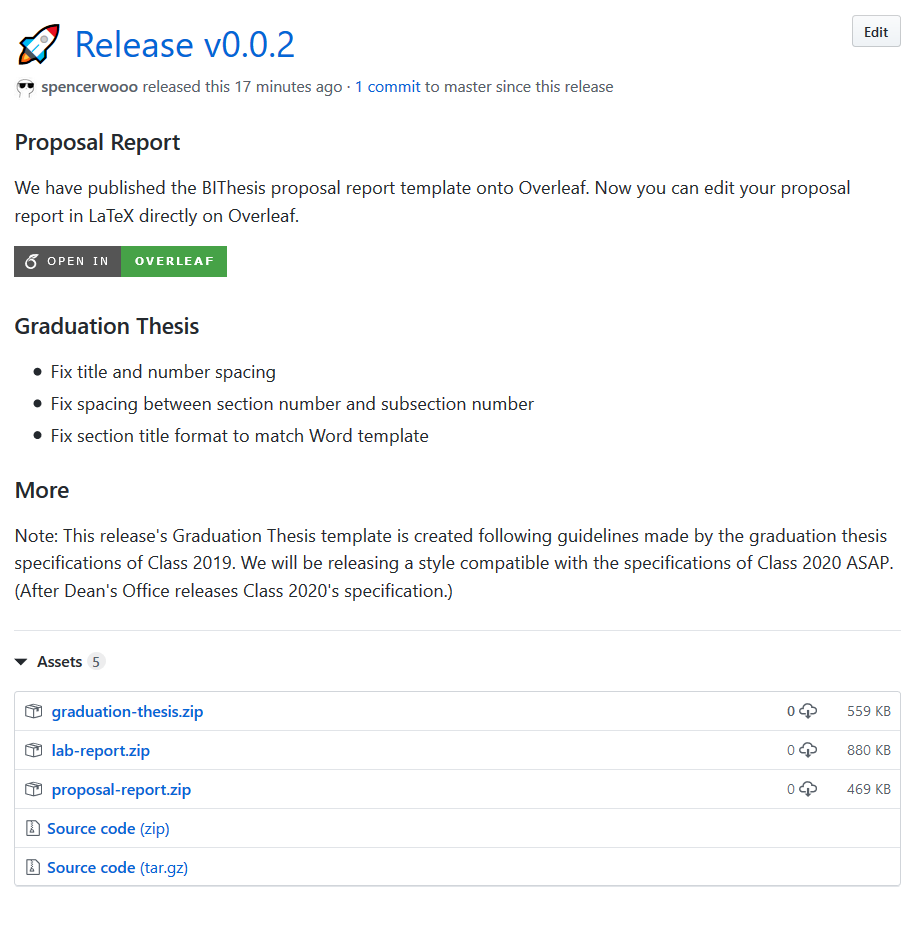
\includegraphics[width=\textwidth]{images/release.png}
  \caption{{\BIThesis} 的 Release 页面}
\end{figure}

根据你的选择,下载其中你所要使用的模板即可。(当然,你也可以直接用 Git 将本项目完整克隆至本地,使用最新版本的模板。)

\subsection{编译模板}

与 Word 不同的是,{\LaTeX} 模板需要我们用合适的工具进行编译,才能生成最终 PDF 文件。我们接下来介绍 {\BIThesis} 中的模板在各个编辑器中的编译方法。

{\BIThesis} 中的模板编译方式大同小异,我们都会使用 \hologo{XeLaTeX}、\hologo{biber} 以及 \texttt{latexmk} 等工具来编译它们。编译 {\BIThesis} 有两种方法:

\begin{enumerate}
  \item 使用 \texttt{xelatex} 配合 \texttt{biber} 进行编译:需要使用“四步走” \texttt{xelatex -> biber -> xelatex -> xelatex} 的编译顺序编译模板,全量编译,编译一次可能花费较长时间
  \item 使用 \texttt{latexmk} 进行编译:只需要使用一次 \texttt{latexmk} 即可编译整个模板,自动识别参考文献编译器,增量编译
\end{enumerate}

这两种编译方式均可以用于编译我们的模板,大家可以综合自己的使用习惯来挑选工具。事实上,后面我们将要介绍的 {\LaTeX} 编辑器,它们背后所使用的编译方法就是运行这里提到的两种编译工具。只是我们需要单独配置编辑器的编译方法,才能让编辑器正确的调用编译方式,编译我们的 {\LaTeX} 文档。

在这里,我挑选了三种常见的 {\LaTeX} 编写环境:

\begin{itemize}
  \item 直接使用“命令行”徒手编写编译
  \item 使用 VS Code 配合 {\LaTeX} Workshop 编写与编译
  \item 使用 \TeX studio 编写与编译
\end{itemize}

我会依次介绍在这三种环境下 {\LaTeX} 编译器配置方法。

\subsubsection{徒手编译}

当然,你完全可以不借助任何编辑器,直接使用“命令行”编译 {\LaTeX} 文档。

\paragraph{使用 \hologo{XeLaTeX} 编译}

如果你使用 \hologo{XeLaTeX} 编译项目,那么你需要按照下面的顺序依次调用 \texttt{xelatex} 与 \texttt{biber} 命令行工具:

\begin{center}
  \begin{tikzpicture}[
    bib/.style={rectangle, draw=ForestGreen!60, fill=ForestGreen!5, very thick, minimum size=8mm},
    xe/.style={rectangle, draw=RubineRed!60, fill=RubineRed!5, very thick, minimum size=8mm},
    ]
  % Nodes
  \node[xe] (xelatex1) {xelatex};
  \node[bib] (biber) [right=of xelatex1] {biber};
  \node[xe] (xelatex2) [right=of biber] {xelatex};
  \node[xe] (xelatex3) [right=of xelatex2] {xelatex};

  % Arrows
  \draw[->] (xelatex1.east) -- (biber.west);
  \draw[->] (biber.east) -- (xelatex2.west);
  \draw[->] (xelatex2.east) -- (xelatex3.west);
  \end{tikzpicture}
\end{center}

比如,编译主文档为 \texttt{main.tex} 的 {\LaTeX} 项目,我们具体的命令为:

\begin{minted}[frame=single,linenos,breaklines]{bash}
  # 第一步 xelatex
  xelatex -no-pdf --interaction=nonstopmode main
  # 第二步 biber
  biber main
  # 第三步 xelatex
  xelatex -no-pdf --interaction=nonstopmode main
  # 第四步 xelatex
  xelatex --interaction=nonstopmode main
\end{minted}

\paragraph{使用 \texttt{latexmk} 编译}

如果你使用 \texttt{latexmk} 编译模板,那么你只需要使用如下的命令即可编译主文件为 \texttt{main.tex} 的 {\LaTeX} 项目:

\begin{minted}[frame=single,linenos,breaklines]{bash}
  # 只需要调用一次 latexmk 工具即可
  latexmk -synctex=1 -interaction=nonstopmode -file-line-error -xelatex main.tex
\end{minted}

\subsubsection{使用 VS Code 撰写与编译 {\LaTeX} 模板}

VS Code 的设置项目可以通过快捷键 \keys{\ctrl \  or\ \cmd + ,} 打开 UI 设置界面,之后点击右上角 \texttt{Open Settings (JSON)} 按钮即可打开相应的 JSON 格式配置文件,我们在这里即可定义 {\LaTeX} 编译工具。其中:

\begin{itemize}
  \item “编译工具”是在 \texttt{"latex-workshop.latex.tools": [ ... ]} 处进行定义,即我们在这里定义每次调用工具 \texttt{xelatex} 或 \texttt{latexmk} 时所执行的命令
  \item “编译工具链”是在 \texttt{"latex-workshop.latex.recipes": [ ... ]} 处进行定义,即我们在这里定义编译整个文档的工具链。对我们的模板第一种编译方式来说,就是定义 \texttt{xelatex -> biber -> xelatex -> xelatex} “四步走”的串联过程
\end{itemize}

\paragraph{使用 \hologo{XeLaTeX} 编译}
这种方法需要调用的工具有:\texttt{xelatex} 和 \texttt{biber}。我们在 VS Code 的设置中加入如下内容定义这两个工具:

\begin{minted}[frame=single,linenos,breaklines]{json}
  "latex-workshop.latex.tools": [
    {
      "name": "xelatex",
      "command": "xelatex",
      "args": [
        "-synctex=1",
        "-interaction=nonstopmode",
        "-file-line-error",
        "-pdf",
        "-outdir=%OUTDIR%",
        "-cd",
        "%DOC%"
      ],
      "env": {}
    },
    {
      "name": "biber",
      "command": "biber",
      "args": [
          "%DOCFILE%"
      ],
      "env": {}
    }
  ]
\end{minted}

用这一方法编译整个文档的工具链串联方法是 \texttt{xelatex -> biber -> xelatex -> xelatex} “四步走”。我们在 VS Code 的设置中加入如下内容定义这个工具链:

\begin{minted}[frame=single,linenos,breaklines]{json}
  "latex-workshop.latex.recipes": [
    {
      "name": "xelatex -> biber -> xelatex * 2",
      "tools": [
        "xelatex",
        "biber",
        "xelatex",
        "xelatex"
      ]
    }
  ]
\end{minted}

\paragraph{使用 \texttt{latexmk} 编译}

这种方法我们只需要使用 \texttt{latexmk} 这一个命令行工具。我们在 VS Code 的设置中添加如下的内容定义这一工具:

\begin{minted}[frame=single,linenos,breaklines]{json}
  "latex-workshop.latex.tools": [
    {
      "name": "latexmk",
      "command": "latexmk",
      "args": [
        "-synctex=1",
        "-interaction=nonstopmode",
        "-file-line-error",
        "-xelatex",
        "-outdir=%OUTDIR%",
        "-cd",
        "%DOC%"
      ],
      "env": {}
    },
  ]
\end{minted}

之后我们再填入下面的内容定义整个工具链(只有一个 \texttt{latexmk}):

\begin{minted}[frame=single,linenos,breaklines]{json}
  "latex-workshop.latex.recipes": [
    {
      "name": "latexmk",
      "tools": [
        "latexmk"
      ]
    },
  ]
\end{minted}

之后,我们使用快捷键 \keys{\ctrl \  or\ \cmd + \shift + P} 打开命令执行栏,并搜索“LaTeX Workshop: Build with recipe”,并选择你所用的 recipe(即上面配置的工具链),即可编译整个 {\LaTeX} 项目。

\begin{figure}[H]
  \centering
  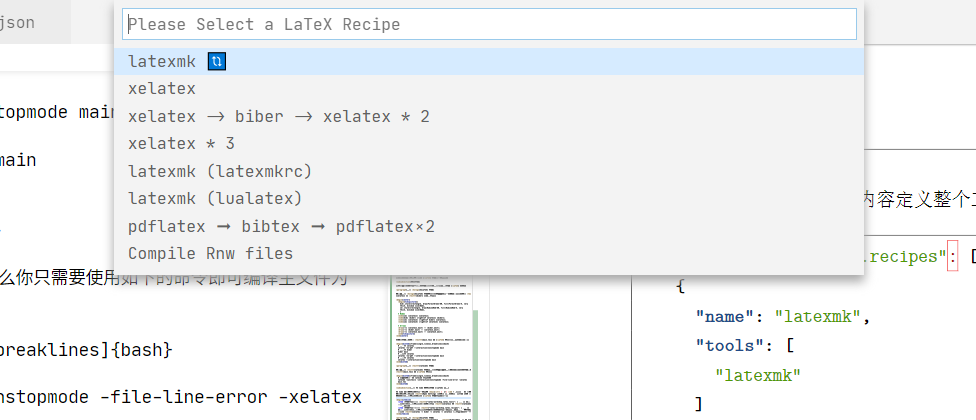
\includegraphics[width=\textwidth]{images/vscode_build_recipe.png}
  \caption{VS Code 挑选 recipe 工具链来编译 {\LaTeX} 项目}
\end{figure}

\subsubsection{使用 \TeX studio 撰写与编译 {\LaTeX} 模板}

\TeX studio 的编译工具大部分已经为我们配置完毕,我们只需要在 \TeX studio 的设置中定义编译所用的编译器即可。在 \TeX studio 中点击“选项 » 设置 TeXstudio”,在打开的窗口中选择“构建”,并在元命令里面将“默认编译器”设置为 \texttt{xelatex} 或 \texttt{latexmk},将默认文献工具设置为 \texttt{biber} 即可。

\begin{figure}[H]
  \centering
  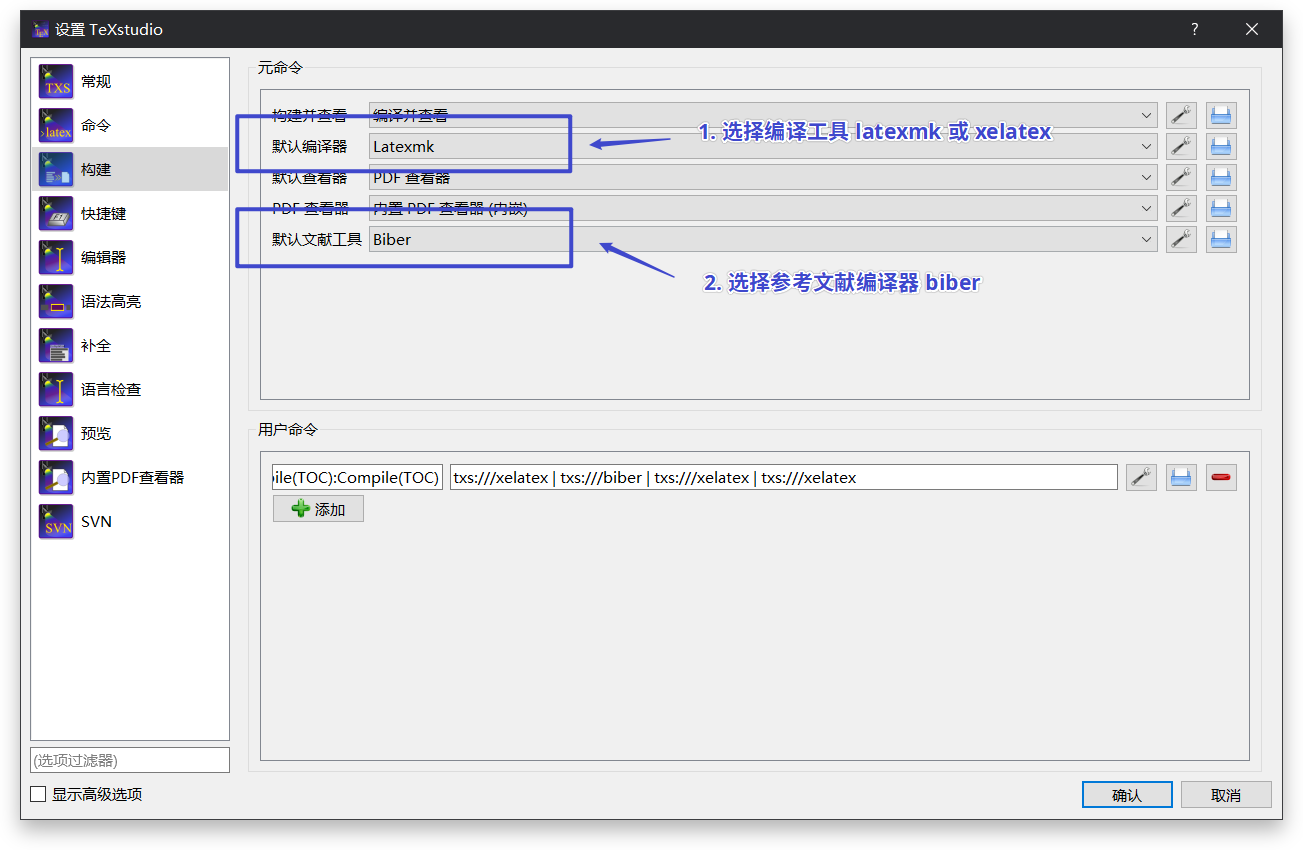
\includegraphics[width=\textwidth]{images/texstudio_build.png}
  \caption{\TeX studio 挑选默认编译器和参考文献工具来编译 {\LaTeX} 项目}
\end{figure}

你可以使用快捷键 \keys{F5} 一键编译与预览 {\LaTeX} 项目。

接下来,请继续在《第 \ref{proposal} 章》、《第 \ref{grad-thesis} 章》和《第 \ref{lab-report} 章》中阅读各个模板的详细模块介绍与用模板撰写论文的具体实施方法。
